\documentclass[main.tex]{subfiles}
\ProvidesPackage{preamble}

\usepackage[nottoc]{tocbibind}
\usepackage[english]{babel}
\usepackage[utf8]{inputenc}
\usepackage[table]{xcolor}
\usepackage[nohead, nomarginpar, margin=1in, foot=.25in]{geometry}
\usepackage{tabularx}
\usepackage{graphicx}
\usepackage{float}
\usepackage[english]{babel}
\usepackage{paralist}
\usepackage{datetime}
\usepackage{afterpage}

\begin{document}

\section{Coding and Integration}

After a brief overview of the project and the project plan, this section will focus on the main technologies used in the project and the rationale behind choosing them. Moving on, we will discuss how these components were integrated and eventually deployed.

\subsection{Overview}

One of the first decision we have made this term was to completely recreate our prototype of Thalia. Firstly, this radical move was the consequence of a new implementation decision (for more detail see \ref{Web Framework}). Secondly, as prototypes are meant to be disposable and are designed only to answer key questions about the system \cite{pragmaticprog}, the proof of concept served its purpose, giving us a chance to refine the structure and the quality of the code.

Despite the risks posed by using an Software Version Control (SVC) Host such as GitHub, we have decided to continue using it as our software development platform. The reasoning behind this builds on the argument developed in our Technical Report \cite{TR_SVC}, which highlights that our, that our Data Processing Module is a completely separate component in our system which none of the other components is able to access. Additionally, we are storing API keys as environment variables in a file that is not tracked by our SVC system, which minimizes the probability of us exposing sensitive data.

TODO talk about API keys and security measures

We have also decided to develop the application with python as our main choice of programming language. Even though this choice seemed obvious from the beginning, we did consider its main benefits, these would be the following:

\begin{itemize}
    \item Python is a high level programming language allowing us to better focus on the application.
    \item A standard choice for prototyping.
    \item Provides superb third party libraries and frameworks for free.
    \item Easy to integrate if we were to choose other languages at some point in our development.
    \item The whole team was already familiar with the language, saving us the precious time needed to learn another programming language.
    \item Our application does not require an unreasonable amount of computation, so there is no need for a more efficient programming language such as C. \ref{BL} \cite{languagescomparison}.
\end{itemize}

We will discuss other technologies used in more detail after the discussion on project planning.

\subsection{Planning}

Early in the inception phase of development we have decided that our goal was not to have fixed responsibilities in our team, allowing everybody to work on each component of the system. This decision has also eased the code review process, as we had no status differences to distort the error-correcting mechanism \cite{statusdifference}. Furthermore, since no team member was the sole developer of a system component, this allowed us to direct comments at the code and not the author \cite{howtoreview}. For these reasons we have decided to follow the Egalitarian Team structure, and make use of the flexibility offered by it. 

Our workflow was centered around the tools provided by GitHub. We used a ticketing system to divide and distribute tasks among team members. These tickets were sometimes given by the team on the weekly meetings, but occasionally they were chosen by the member proposing the feature or change. Our goal with this approach was to divide larger jobs into smaller tasks. 

A typical ticket in our project was an encapsulation of a user story, as it consisted of a title, a one liner, value, acceptance criteria, and sub tasks. In the first half of development we also used effort-oriented metrics, called story points to measure the amount of work but we decided to abandon this aspect. An example of a ticket can be seen on \figurename{\ref{Ticket}}.

\begin{figure}[H]
   \centering
   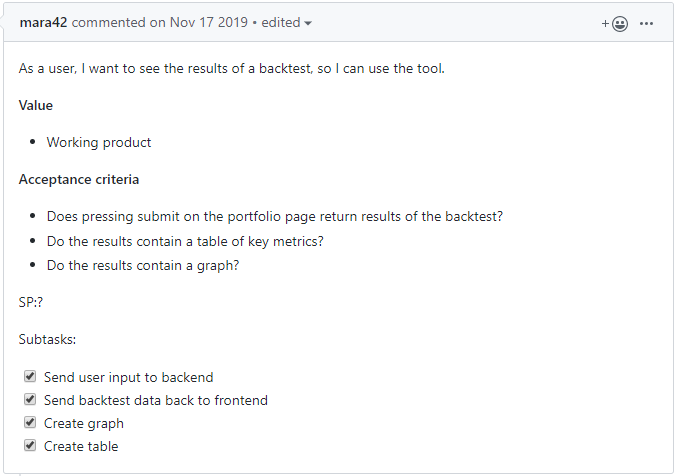
\includegraphics[scale=0.7]{05Coding/05Pictures/ticket.png}
   \caption{Ticket Example}
   \label{Ticket}
\end{figure}

TODO update git stats

Throughout the whole project we had a total of 110 tickets, and 71 pull requests. The following graph also shows the number of contributions to master, excluding merge commits.

\begin{figure}[H]
   \centering
   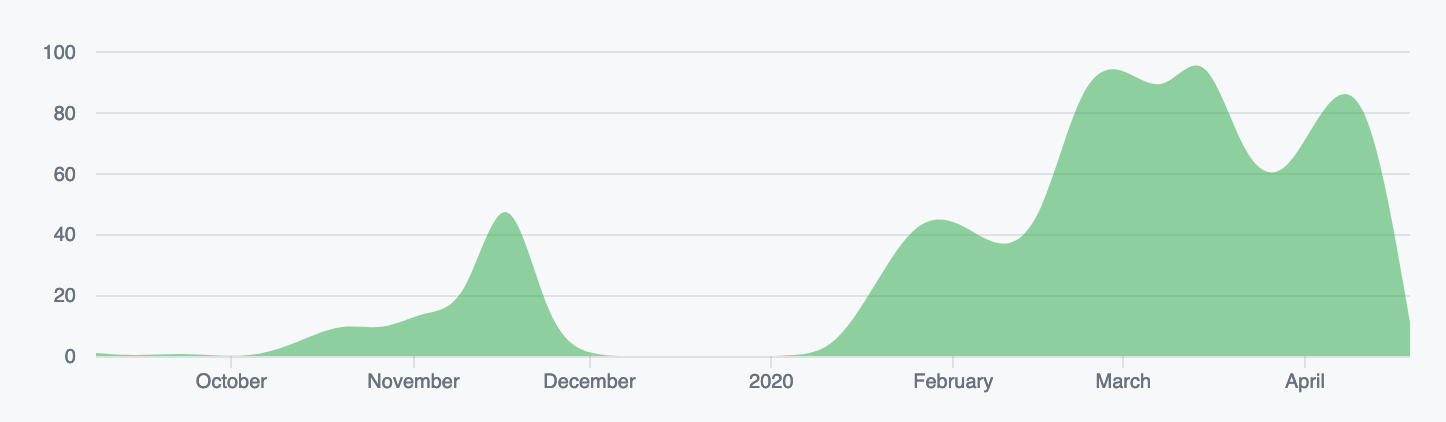
\includegraphics[scale=0.8]{05Coding/05Pictures/contributions.png}
   \caption{Contributions to the Master branch}
\end{figure}

Nevertheless, this was not always achievable especially in the beginning of the development when more crucial components of the systems were developed. In these cases, we assigned the ticket to a pair, or group of people. This approach achieved the following:

\begin{itemize}
    \item Improved the overall code quality and fastened production \cite{pairprogramming}.
    \item Minimised review time on the long run.
    \item Distributed the knowledge of large system components amongst a few people instead of one.
    \item Eased introducing the new team member to the project.
\end{itemize}

In addition, we also had a scrum board as an overview for the ongoing tickets. Although in the Scrum community there are ongoing discussions about the benefits of a physical scrum board over an online one \cite{physicalscrum}, given no actual workplace this was not possible to achieve. This allowed us to see which tickets needed to be reviewed and which were ready to be merged. The tickets/cards were distributed into columns, such as To do, In progress, Review in progress, Review complete and Finished. A truncated picture of this scrum board can be seen on figure \figurename{\ref{Scrum}}.

\begin{figure}[H]
   \centering
   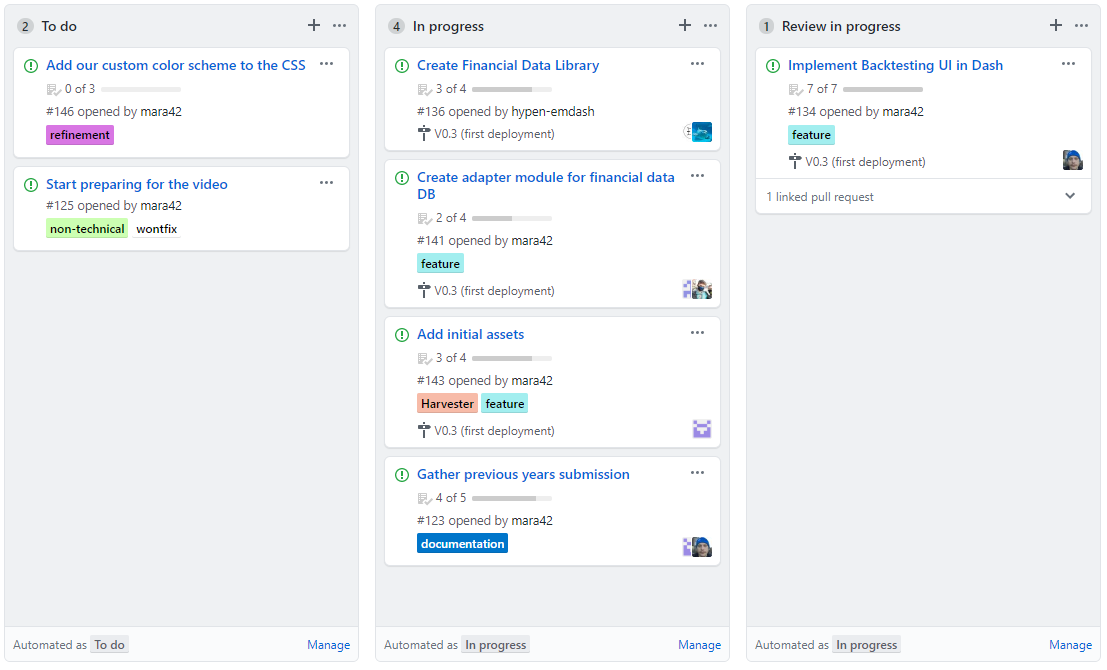
\includegraphics[scale=0.55]{05Coding/05Pictures/scrumboard.png}
   \caption{Scrum board - truncated}
   \label{Scrum}
\end{figure}

The workflow then largely depended on the task at hand and the person working on it. It was up to them if they met for pair-programming, or chose to work individually. In the beginning we all agreed on the developing environment and coding standards (for a detailed analysis see the later section \ref{Coding Standards}). Since this report was a relevant portion of the workload, we decided to treat it as code. The report was written in \LaTeX, first creating the overall structure of the document with a main.tex compiling the sections together. This let us to work on different sections separately just like features in our software. 

Regardless of the nature of the ticket, the week, or in case of some larger tasks, two weeks, ended by the creator indicating that the changes were ready to be integrated. This was done by publishing the changes and creating a new pull request, pushing the changes onto the master branch. To ensure code quality, we set up a continuous integration (CI) environment (more on that in \ref{Coding Standards}). After all checks have passed, the changes were successfully integrated into the code base.

\subsection{Schedule}
As mentioned in our Technical Report, we introduced some milestones or releases for our product based on incremental sets of features. This was done to help us stay on track with development. The roadmap based on this schedule can be seen on \figurename{\ref{Roadmap}}.

\begin{figure}[H]
   \centering
   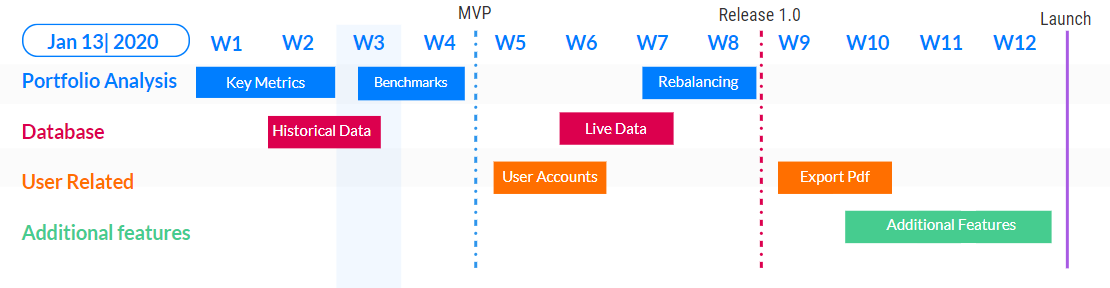
\includegraphics[scale=0.55]{05Coding/05Pictures/initial_roadmap.png}
   \caption{Technical Report: Roadmap - revisited}
   \label{Roadmap}
\end{figure}

TODO retrospective on schedule

\subsection{Key Implementation Decisions}

Let us now discuss the main technologies used in our project, these can be categorised as follows:
\subsubsection{Web Framework}
\label{Web Framework}
Choosing the right web framework was more controversial than originally planed. The two major options for Python are Django and Flask. Although we decided to use Django for our MVP in the first semester, we had to spend a significant portion of the time available learning the framework, so we had to decide whether we were going to stick with it or learn Flask. In the end, we opted to go with Flask for the following reasons:

\begin{itemize}
    \item Django has one architecture that all projects must share, and we have designed the architecture for our project ourselves. While neither architecture is wrong, the two are not compatible. Flask, on the other hand, is structure-agnostic, so we can lay out the code as we see fit.

    \item Flask comes with the bare minimum for web-development, which means that we don't need to manage the complexity of any feature we're not using. Django has a more complete feature-set from the beginning. This would be desirable in a large web application, but introduces significant overhead in our case, where the website has only a handful of pages.
    
    \item Django all but insists on using its ORM for all database interaction, while we plan to have a more manual approach.
    
    \item Our concerns were also confirmed by more experienced web-developers, suggesting simpler alternatives.
\end{itemize}

As stated this decision has contributed to the opportunity to recreate the basis of our application, and to apply what we have learnt from our prototype. 

\iffalse
Sources:
https://www.djangoproject.com/

https://flask.palletsprojects.com/en/1.1.x/

https://www.codementor.io/@garethdwyer/flask-vs-django-why-flask-might-be-better-4xs7mdf8v

http://ddi-dev.com/blog/programming/django-vs-flask-which-better-your-web-app/

https://coderseye.com/django-vs-flask
\fi

\subsubsection{GUI}
\subsubsection{Business Logic}
\label{BL}
\subsubsection{Database \& Finda}
\subsubsection{Harvester}

\subsection{Integration}
\label{Coding Standards}
 
 Writing well documented and good quality code is one thing, but making sure it all works together as a whole is a completely different story. In the first term, many hours have been wasted on trying to integrate different components of the system which did not want to fit together. Even then we had some DevOps tools in place \cite{DevOps}, but considering that we had to produce significantly less code and more documentation last term, this was not a priority. 
 
 Starting afresh the coming term, we have decided to set up the development environment again. Upon opening the setup.py file, we see a list of required libraries, and the following two lines of code:

\begin{lstlisting}[language=Python, caption=setup.py - Development environment, label=lst:Development_env]
"""A setuptools based setup module."""
from os import path

from setuptools import find_packages, setup

here = path.abspath(path.dirname(__file__))

install_requires = [
    "flask",
    "flask-login >= 0.5",
    "flask-migrate",
    "flask-wtf",
    "pandas",
    "dash",
]


tests_require = ["pytest", "coverage"]

extras_require = {"dev": ["black", "flake8", "pre-commit"], "test": tests_require}

setup(
    name="Thalia",
    version="0.2.0",
    packages=find_packages(),
    install_requires=install_requires,
    extras_require=extras_require,
)
\end{lstlisting}

One of the first decisions we had to make, is to decide on a standards coding style. This is exactly what flake8 is for, which we can see amongst the extras in the code snippet above. The original documentation of flake8 defines it as " [...] is a command-line utility for enforcing style consistency across Python projects. By default it includes lint checks provided by the PyFlakes project, PEP-0008 inspired style checks provided by the PyCodeStyle project, and McCabe complexity checking provided by the McCabe project" \cite{flake8}. However, as many other developers we also decided to redefine the maximum line-length from 79 to 88 as we found this convention a hindrance. 

Another tool used for enforcing uniform style was the black auto-formatter for Python \cite{black}, which formatted the code for us upon every save if enabled, and also when commiting code. This has been achieved by the use of githooks \cite{githooks}, which are programs that are triggered upon certain git actions. For this we needed the pre-commit package for setting up these actions and writing the configuration file. This ensured that both flake8 and black have been run before publishing changes.

\subsubsection{Continuous Integration}
\label{Continuous Integration}

Many studies have investigated the positive effects of developing in a continuous integration (CI) environment \cite{CI_1}, \cite{CI_2}. Regardless of the exact implementation, its obvious benefit is that it provides security and uniformity for projects. We already made some steps to achieve a uniform style, but had no means to know whether the code published has been also passed its tests. Note in this section we will only discuss testing as a part of CI and not the testing strategy, for that see the section \ref{Testing}.

Another important part of the DevOps toolchain is the use of containers, which is what Docker helps to achieve \cite{Docker}. Docker helps developers focus on writing code rather than worrying about the system the application will be running on, and also helps to reveal dependency and library issues. As Docker is open source, there are many free to use docker images available online \cite{Docker Images}. When choosing the CI environment, Docker support was one of the main requirements. 

The most promising candidate for this was CircleCI \cite{CircleCI}, which is a cloud-based system with first-class Docker support and a free trial. After connecting our GitHub repository to CircleCI, and setting up a configuration, CircleCI now does the following on every pull-request:

\begin{enumerate}
    \item Sets up a clean container or virtual machine for the code.
    \item Checks previously cached requirements. 
    \item Installs the requirements from requirements.txt
    \item Caches the requirements for faster performance.
    \item Clones the branch needed to be merged.
    \item Runs flake8 one last time and saves results.
    \item Runs tests and saves results. 
    \item Deploys the master branch to Heroku, see \ref{Continuous Deployment}
\end{enumerate}

The outcome of these steps is visible on CircleCI, but more importantly also on GitHub, and it refuses to merge if failing test (or no tests) have been found. 

 \begin{figure}[H]
   \centering
   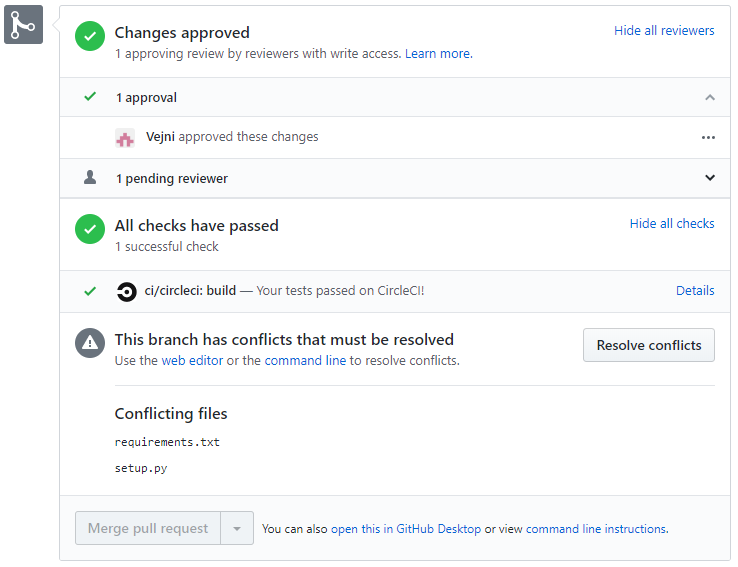
\includegraphics[scale=0.6]{05Coding/05Pictures/circleCI.png}
   \caption{CircleCI on GitHub}
   \label{CircleCI}
\end{figure}

With the help of these steps and CircleCI we managed to ensure that the code written is uniform and of good quality. It significantly reduced the time needed for integrating and code reviewing. The last step was now to deploy the system. 

\subsection{Hosting and Deployment}
\label{Continuous Deployment}

An overview over the literature covering reveals a plethora of different strategies for deploying and hosting web applicaitons \cite{ConnollyFundamentals}. Our decision of how to choose among them involved the following considerations:

\begin{itemize}
	\item Price - since we have severe budget constraints, we were looking for a cheap hosting solution
	\item CircleCI support - The target host should be supported by CircleCI natively to ease development of a continuous deployment (CD) pipeline
\end{itemize}

The upfront cost of buying physical servers ruled it out as an option for us. Thus, we turned our attention to using a solution that involved deployment to a virtual machine in the Cloud. Many providers for such a service exist, including Amazon Web Services \cite{AWS} and Microsoft Azure \cite{Azure}. While these would provide us with extensive control over the hosting process, their use involves a lot of complexity that seemed unnecessary for the intial rollout of a simple application such as Thalia.

Due to native CircleCI support and a free tier service, we ended up choosing Heroku \cite{Heroku} as our initial hosting provider. This enables us to host our application for free in the initial stages of development while providing ample opportunity for horizontal and vertical scaling later on, if it is required.

The benefits of using continuous deployment have been well established for multiple years and involve "the ability to get faster feedback, the ability to deploy more often to keep customers satisfied, and improved quality and productivity" \cite{CDBenefits}. Using Heroku in combination with CircleCI, our CD pipeline involves the following simple steps:

\begin{enumerate}
	\item Upon commits to the master branch on GitHub, CircleCI triggers a workflow.
	\item The workflow first executes the steps listed in \ref{Continuous Integration} to ensure the validity of the current codebase state.
	\item If this step is successful, the master branch is pushed to a remote repository recognized by Heroku via git.
	\item Heroku executes the Procfile script stored in the root of our project to start the application using a gunicorn web server \cite{Gunicorn}.
\end{enumerate}

Our deployment process is thus fully automized and immune to failing tests, as it will only complete successfully if the application is in a correct state.

\end{document}
